%%===========================================================%%
%%                                                           %%
%%          RpTrigEfficiencySystematicsAppendix              %%
%%                                                           %%
%%===========================================================%%

\chapter{RP trigger counters efficiency comparison between data and MC}\label{appendix:rpTrigEffSyst}%\vspace{-26pt}




%---------------------------
\begin{figure}[h]%\vspace{-34pt}
	\centering
	\parbox{0.4725\textwidth}{
		\centering
		\includegraphics[width=\linewidth,page=2]{graphics/systematicsEfficiency/RpSyst/relativeTriggerEff2D_pxpy.pdf}%\vspace{-12pt}
	}
	\quad
	\parbox{0.4725\textwidth}{
		\centering\vspace*{-100pt}
		\caption[Coparison of estimated RP trigger counter efficiency in 2D (detector E2U).]%
    {Sample comparison of RP trigger counter efficiency (detector E2U) in the data (top panel) and embedded MC (middle panel) estimated with the method described in Sec.~\ref{sec:rpTriggerEffSystematics} as a function of $(p_{x},p_{y})$ of a proton track. Lower pad shows the difference between efficiency extracted from the data and MC. Hatched orange area marks bins without any entries (efficiency incalculable).% 
    }
	}
	\label{fig:relativeRpRecoEff_E2U}
\end{figure}
%---------------------------



%---------------------------
\begin{figure}[h]%\vspace{-34pt}
	\centering
	\parbox{0.4725\textwidth}{
		\centering
		\includegraphics[width=\linewidth,page=3]{graphics/systematicsEfficiency/RpSyst/relativeTriggerEff2D_pxpy.pdf}%\vspace{-12pt}
	}
	\quad
	\parbox{0.4725\textwidth}{
		\centering\vspace*{-100pt}
		\caption[Coparison of estimated RP trigger counter efficiency in 2D (detector E1D).]%
    {Sample comparison of RP trigger counter efficiency (detector E1D) in the data (top panel) and embedded MC (middle panel) estimated with the method described in Sec.~\ref{sec:rpTriggerEffSystematics} as a function of $(p_{x},p_{y})$ of a proton track. Lower pad shows the difference between efficiency extracted from the data and MC. Hatched orange area marks bins without any entries (efficiency incalculable).% 
    }
	}
	\label{fig:relativeRpRecoEff_E1D}
\end{figure}
%---------------------------




%---------------------------
\begin{figure}[h]%\vspace{-34pt}
	\centering
	\parbox{0.4725\textwidth}{
		\centering
		\includegraphics[width=\linewidth,page=4]{graphics/systematicsEfficiency/RpSyst/relativeTriggerEff2D_pxpy.pdf}%\vspace{-12pt}
	}
	\quad
	\parbox{0.4725\textwidth}{
		\centering\vspace*{-100pt}
		\caption[Coparison of estimated RP trigger counter efficiency in 2D (detector E2D).]%
    {Sample comparison of RP trigger counter efficiency (detector E2D) in the data (top panel) and embedded MC (middle panel) estimated with the method described in Sec.~\ref{sec:rpTriggerEffSystematics} as a function of $(p_{x},p_{y})$ of a proton track. Lower pad shows the difference between efficiency extracted from the data and MC. Hatched orange area marks bins without any entries (efficiency incalculable).% 
    }
	}
	\label{fig:relativeRpRecoEff_E2D}
\end{figure}
%---------------------------




%---------------------------
\begin{figure}[h]%\vspace{-34pt}
	\centering
	\parbox{0.4725\textwidth}{
		\centering
		\includegraphics[width=\linewidth,page=5]{graphics/systematicsEfficiency/RpSyst/relativeTriggerEff2D_pxpy.pdf}%\vspace{-12pt}
	}
	\quad
	\parbox{0.4725\textwidth}{
		\centering\vspace*{-100pt}
		\caption[Coparison of estimated RP trigger counter efficiency in 2D (detector W1U).]%
    {Sample comparison of RP trigger counter efficiency (detector W1U) in the data (top panel) and embedded MC (middle panel) estimated with the method described in Sec.~\ref{sec:rpTriggerEffSystematics} as a function of $(p_{x},p_{y})$ of a proton track. Lower pad shows the difference between efficiency extracted from the data and MC. Hatched orange area marks bins without any entries (efficiency incalculable).% 
    }
	}
	\label{fig:relativeRpRecoEff_W1U}
\end{figure}
%---------------------------




%---------------------------
\begin{figure}[h]%\vspace{-34pt}
	\centering
	\parbox{0.4725\textwidth}{
		\centering
		\includegraphics[width=\linewidth,page=3]{graphics/systematicsEfficiency/RpSyst/relativeTriggerEff2D_pxpy.pdf}%\vspace{-12pt}
	}
	\quad
	\parbox{0.4725\textwidth}{
		\centering\vspace*{-100pt}
		\caption[Coparison of estimated RP trigger counter efficiency in 2D (detector E1D).]%
    {Sample comparison of RP trigger counter efficiency (detector E1D) in the data (top panel) and embedded MC (middle panel) estimated with the method described in Sec.~\ref{sec:rpTriggerEffSystematics} as a function of $(p_{x},p_{y})$ of a proton track. Lower pad shows the difference between efficiency extracted from the data and MC. Hatched orange area marks bins without any entries (efficiency incalculable).% 
    }
	}
	\label{fig:relativeRpRecoEff_E1D}
\end{figure}
%---------------------------




%---------------------------
\begin{figure}[h]%\vspace{-34pt}
	\centering
	\parbox{0.4725\textwidth}{
		\centering
		\includegraphics[width=\linewidth,page=6]{graphics/systematicsEfficiency/RpSyst/relativeTriggerEff2D_pxpy.pdf}%\vspace{-12pt}
	}
	\quad
	\parbox{0.4725\textwidth}{
		\centering\vspace*{-100pt}
		\caption[Coparison of estimated RP trigger counter efficiency in 2D (detector W2U).]%
    {Sample comparison of RP trigger counter efficiency (detector W2U) in the data (top panel) and embedded MC (middle panel) estimated with the method described in Sec.~\ref{sec:rpTriggerEffSystematics} as a function of $(p_{x},p_{y})$ of a proton track. Lower pad shows the difference between efficiency extracted from the data and MC. Hatched orange area marks bins without any entries (efficiency incalculable).% 
    }
	}
	\label{fig:relativeRpRecoEff_W2U}
\end{figure}
%---------------------------




%---------------------------
\begin{figure}[h]%\vspace{-34pt}
	\centering
	\parbox{0.4725\textwidth}{
		\centering
		\includegraphics[width=\linewidth,page=7]{graphics/systematicsEfficiency/RpSyst/relativeTriggerEff2D_pxpy.pdf}%\vspace{-12pt}
	}
	\quad
	\parbox{0.4725\textwidth}{
		\centering\vspace*{-100pt}
		\caption[Coparison of estimated RP trigger counter efficiency in 2D (detector W1D).]%
    {Sample comparison of RP trigger counter efficiency (detector W1D) in the data (top panel) and embedded MC (middle panel) estimated with the method described in Sec.~\ref{sec:rpTriggerEffSystematics} as a function of $(p_{x},p_{y})$ of a proton track. Lower pad shows the difference between efficiency extracted from the data and MC. Hatched orange area marks bins without any entries (efficiency incalculable).% 
    }
	}
	\label{fig:relativeRpRecoEff_W1D}
\end{figure}
%---------------------------




%---------------------------
\begin{figure}[h]%\vspace{-34pt}
	\centering
	\parbox{0.4725\textwidth}{
		\centering
		\includegraphics[width=\linewidth,page=8]{graphics/systematicsEfficiency/RpSyst/relativeTriggerEff2D_pxpy.pdf}%\vspace{-12pt}
	}
	\quad
	\parbox{0.4725\textwidth}{
		\centering\vspace*{-100pt}
		\caption[Coparison of estimated RP trigger counter efficiency in 2D (detector W2D).]%
    {Sample comparison of RP trigger counter efficiency (detector W2D) in the data (top panel) and embedded MC (middle panel) estimated with the method described in Sec.~\ref{sec:rpTriggerEffSystematics} as a function of $(p_{x},p_{y})$ of a proton track. Lower pad shows the difference between efficiency extracted from the data and MC. Hatched orange area marks bins without any entries (efficiency incalculable).% 
    }
	}
	\label{fig:relativeRpRecoEff_W2D}
\end{figure}
%---------------------------

